\begin{figure}[ht]
\centering
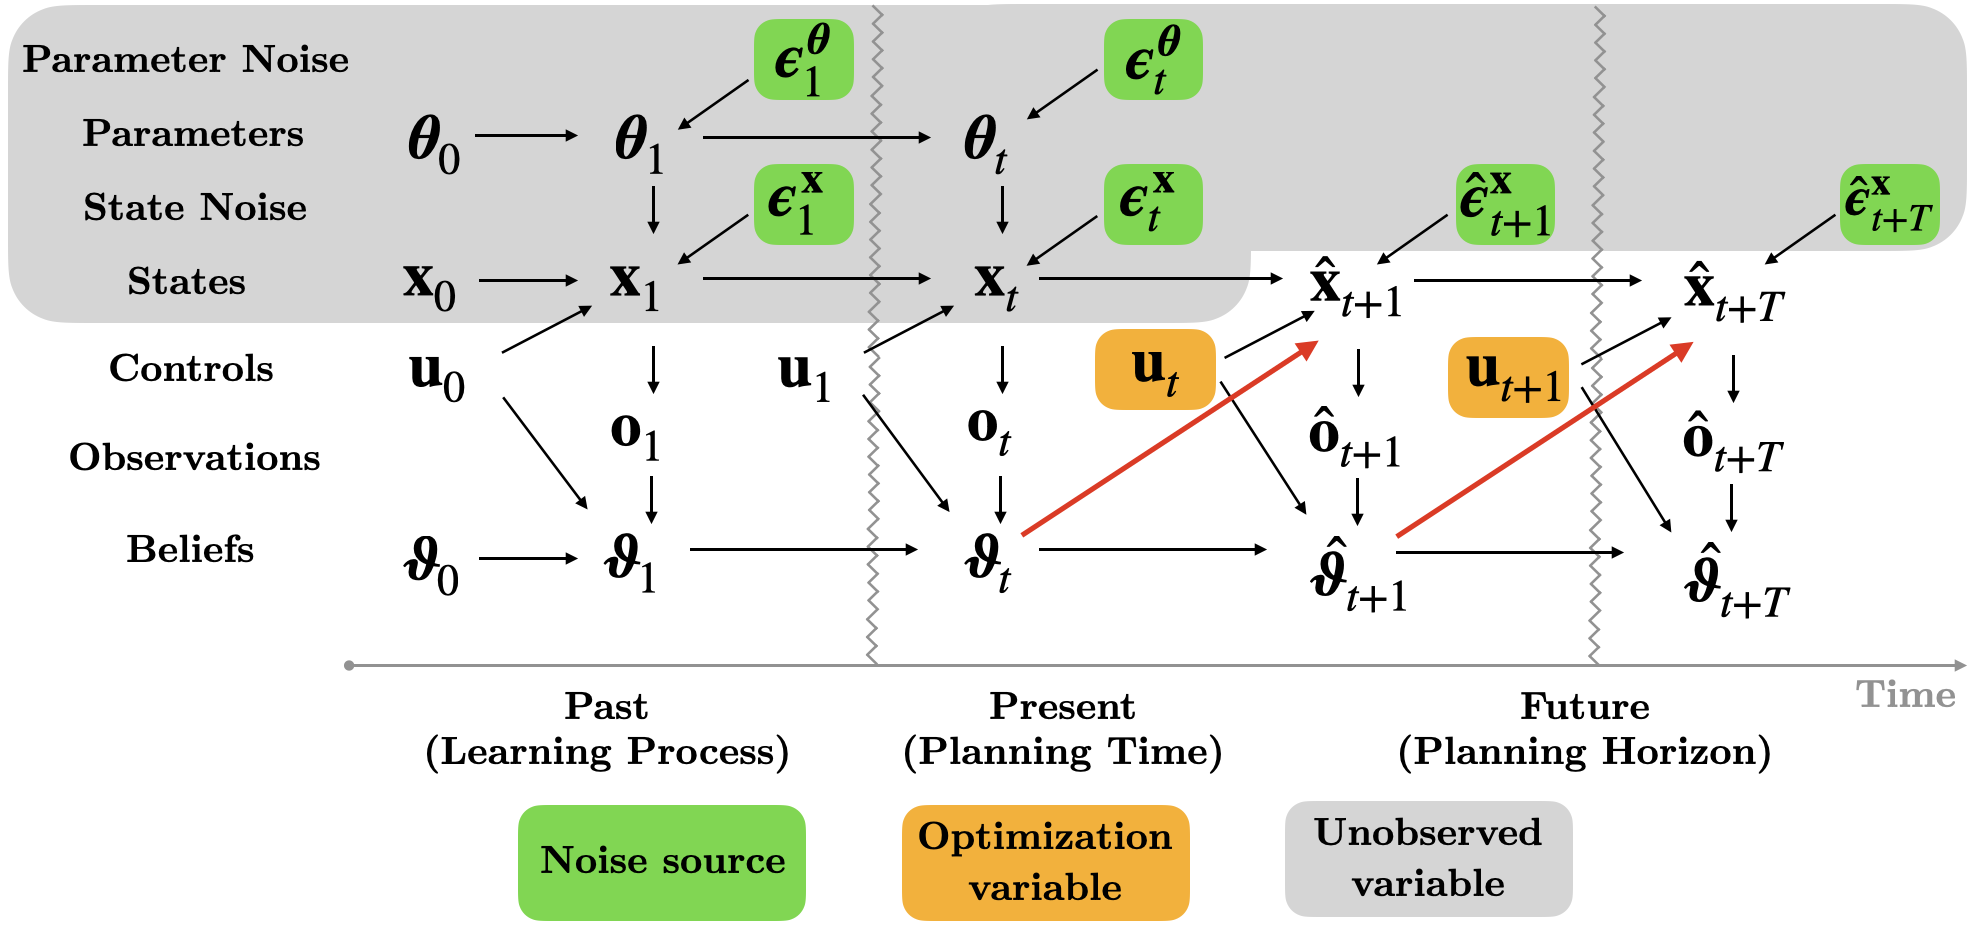
\includegraphics[width=1.0\linewidth]{figures/causal.png}
\caption{Causal graph for states $\state_\timeindex$, observations $\observation_\timeindex$, controls $\control_\timeindex$, parameters $\params_\timeindex$, beliefs $\belief_\timeindex$, and noise $\noise_\timeindex$. 
Planning is done at time $\timestart$ for a planning horizon $\horizon$. 
Zigzag lines denote axis breaks.
A variable with a hat denotes a prediction made during planning.
Red lines emphasize the causal dependencies between states and beliefs during prediction: since the true parameters are not available, the states must be predicted using the latest dynamics parameters belief.}
\label{fig:causal}
\vspace{-10pt}
\end{figure}


\section{Introduction}
An agent operating in an unknown dynamical system must learn it from observations. 
It can do so passively, by simply collecting data as it pursues other cost, or actively, by seeking maximally informative observations. 
In this paper we focus on the problem of active information gathering, which is important because collecting information-dense observations reduces time, energy, and risk during exploration.

The problem of information gathering is hard for two reasons. 
First, it requires evaluating complex nested expectations to compute how future uncertainty changes as a function of planned actions \cite{bar1974dual,klenske2016dual}.
Second, existing formalizations do not cleanly expose the causal dependencies between beliefs, controls, and states. 
Consequently, existing methods rely upon information-gathering costs derived from specific problem structures. 

In this work, we present a unifying framework that cleanly exposes the causal dependencies between parameters, states, controls, observations, beliefs, and predicted beliefs (see \cref{fig:causal} for a visualization) \textit{without} committing to a specific dynamics model type, belief update procedure, belief dynamics model, observation model, or planning procedure \textbf{(Contribution 1, \cref{sec:contribution1})}.
Then we derive a general information-gathering cost based on directed information \cite{massey1990causality}, which we prove captures existing approaches based on mutual information, cf. \cite{sukhija2023optimistic, buisson2020actively,lew2022safe,krause2007nonmyopic,zimmer2018safe,abraham2019active,vantilborgh2025dual,davydov2024first, palafox2025info} for examples, \textbf{(Contribution 2, \cref{sec:contribution2})}.
Equipped with this framework, we derive an explicit connection between information gathering and uncertainty reduction in linearized Bayesian estimation, providing a measure of theoretical justification for mutual information that prior frameworks could not easily expose 
\textbf{(Contribution 3, \cref{sec:contribution3})}.
Finally, we present experiments on single-agent and multi-agent settings, showcasing the practical utility of our theoretical framework \textbf{(Contribution 4, \cref{sec:contribution4})}.
Moving forward, our framework opens the door for new combinations of learning and planning components that prior formalisms could not express.